%%%%%%%%%%%%%%%%%%%%%%%%%%%%%%%%%%%%%%%%%%%%%%%%%%%%%%%%%%%%%%%%%%%%%%%%
% Escuela Politécnica Superior de la Universidad de Alicante
% Realizado por: Jose Manuel Requena Plens
% Contacto: info@jmrplens.com / Telegram:@jmrplens
%%%%%%%%%%%%%%%%%%%%%%%%%%%%%%%%%%%%%%%%%%%%%%%%%%%%%%%%%%%%%%%%%%%%%%%%

\pgfkeys{/pgf/number format/.cd,1000 sep={\,}}
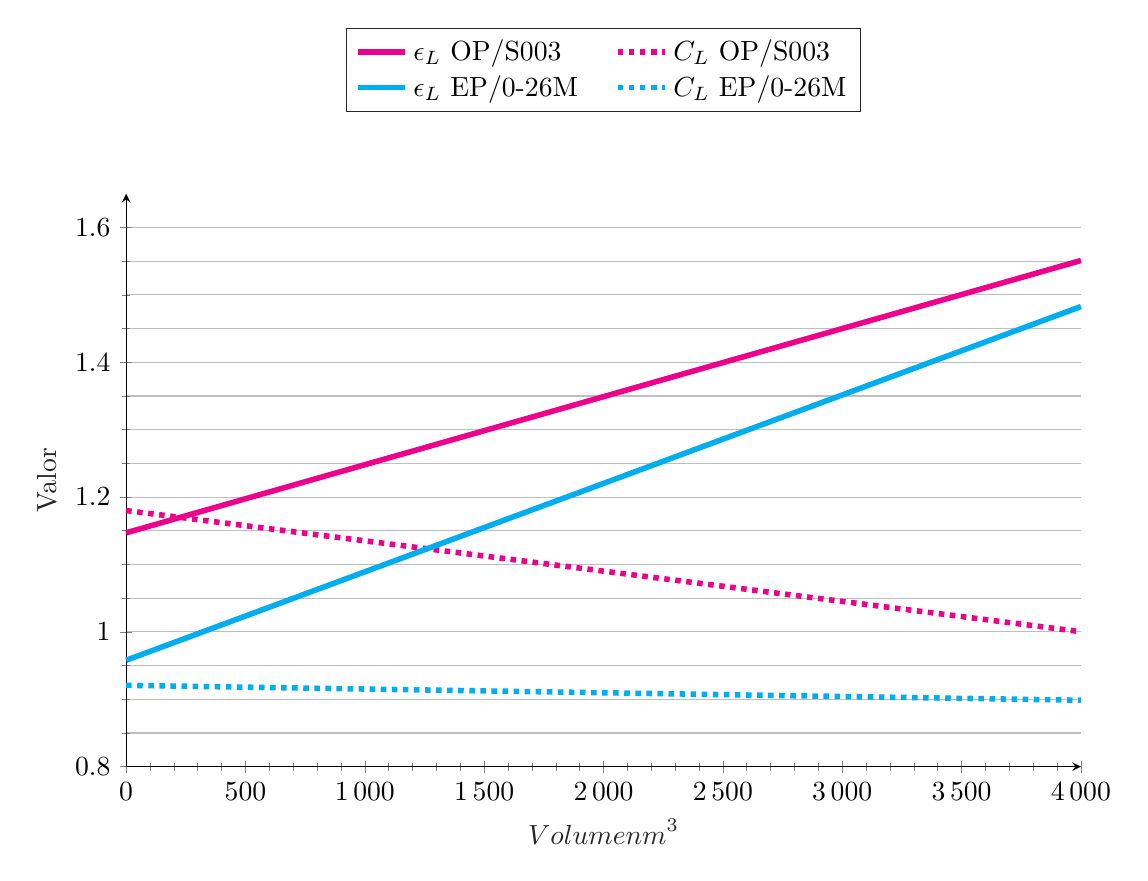
\begin{tikzpicture}

\begin{axis}[%
width=\textwidth,
height=0.6\textwidth,
at={(0\textwidth,0\textwidth)},
scale only axis,
xmin=0,
xmax=4000,
clip=false,
axis y line=left,
axis x line=bottom,
xlabel style={font=\color{white!15!black}},
xlabel={$\text{Volumen m}^\text{3}$},
ymin=0.8,
ymax=1.65,
minor x tick num= 4,
minor y tick num= 3,
yminorgrids,
ymajorgrids,
ylabel style={font=\color{white!15!black}},
ylabel={Valor},
axis background/.style={fill=white},
legend columns=2,
legend style={legend cell align=left, align=left, draw=white!15!black,at={(0.5,1.29)},anchor=north,/tikz/every even column/.append style={column sep=0.4cm}}
]

\addplot [color=magenta, line width=2.0pt,domain=0:4000, samples=10]
{0.000101*x+1.147};
\addlegendentry{$\epsilon_L$ OP/S003}

\addplot [color=magenta, dotted,line width=2.0pt,domain=0:4000, samples=10]
{-4.494e-05*x+1.18};
\addlegendentry{$C_L$ OP/S003}

\addplot [color=cyan, line width=2.0pt,domain=0:4000, samples=10]
{0.0001312*x+0.9579};
\addlegendentry{$\epsilon_L$ EP/0-26M}

\addplot [color=cyan, dotted,line width=2.0pt,domain=0:4000, samples=10]
{-5.532e-06*x+0.9207};
\addlegendentry{$C_L$ EP/0-26M}

\end{axis}
\end{tikzpicture}%